
    %                     %            %
    %                                  %
    %                                  %
   %%%    %%%%   %%%%%   %%           %%%    %%%%  %    %
    %    %    % %         %            %    %    %  %  %
    %    %%%%%%  %%%%     %            %    %%%%%%   %%
    %    %           %    %            %    %        %%
    %    %           %    %     %%     %    %       %  %
     %%   %%%%% %%%%%    %%%    %%      %%   %%%%% %    %



         %%%%%%%%%%%%%%%%%%%%%%%%%%%%%%%%%%%%%%%%
         %                                      %
         %  "Scheletro" di una tesi di laurea   %
         %           (in Ingegneria)            %
         %      dell'Universita` di Udine       %
         %                                      %
         %%%%%%%%%%%%%%%%%%%%%%%%%%%%%%%%%%%%%%%%

            %%%%%%%%%%%%%%%%%%%%%%%%%%%%%%%%%%
            %    Autore: Gianluca Gorni      %
            % Modificato (per ingegneria) da:%
            %       Nicola Driutti           %
            %%%%%%%%%%%%%%%%%%%%%%%%%%%%%%%%%%

   %%%%%%%%%%%%%%%%%%%%%%%%%%%%%%%%%%%%%%%%%%%%%%%%%
   %%%%%  Ultima modifica:  8 febbraio 2006    %%%%%
   %%%%%%%%%%%%%%%%%%%%%%%%%%%%%%%%%%%%%%%%%%%%%%%%%



                                 %            %%
                                 %             %
   %%%%  % %%   %%%   %%%% %%%%  %%%%   %%%    %    %%%
   %   % %%  % %   % %   % % % % %   % %   %   %   %   %
   %   % %     %%%%% %   % % % % %   % %   %   %   %   %
   %   % %     %     %  %% % % % %   % %   %   %   %   %
   %%%%  %      %%%%  %% % % % % %%%%   %%%   %%%   %%%
   %
   %




  %%%%%%%%%%%%%%%%%%%%%%%%%%%%%%%%%%%%%%%%%%%%%%%%%%%%%%%%%
  % Usare una versione di LaTeX con sillabazione italiana %
  %%%%%%%%%%%%%%%%%%%%%%%%%%%%%%%%%%%%%%%%%%%%%%%%%%%%%%%%%

\documentclass[12pt,a4paper,twoside,italian]{book}

% Usare "oneside" invece di "twoside"
% nelle bozze, per risparmiare carta:
% "twoside" produce diverse pagine bianche
% alla fine dei capitoli.

                    %%%%%%%%%%%%%%%%%%%%%%%%%%%%%%%%
                    %         inputenc             %
                    %  Usare l'opzione "latin1"    %
                    %  se si vogliono scrivere     %
                    %  lettere accentate da        %
                    %  tastiera su Windows o Unix  %
                    %%%%%%%%%%%%%%%%%%%%%%%%%%%%%%%%

%\usepackage[latin1]{inputenc}

       %%%%%%%%%%%%%%%%%%%%%%%%%%%%%%%%%%%%%%%%%%%%%%
       %                  babel                     %
       % Pacchetto tipico per una tesi in italiano. %
       %%%%%%%%%%%%%%%%%%%%%%%%%%%%%%%%%%%%%%%%%%%%%%


\usepackage{babel}

   %%%%%%%%%%%%%%%%%%%%%%%%%%%%%%%%%%%%%%%%%%%%%%%%%%%%%%%%%%%%
   % Se nella tesi si inseriscono dei passi in un'altra       %
   % lingua (inglese, per fissare le idee), si puo' istruire  %
   % il TeX di sillabare quella parte di testo con le regole  %
   % inglesi, invece che italiane. A questo scopo basta       %
   % scrivere                                                 %
   %                                                          %
   %    \usepackage[english,italian]{babel}                   %
   %                                                          %
   % al posto di \usepackage[italian]{babel},                 %
   % dopodiche la sillabazione sara' italiana fintanto che    %
   % non si incontra il comando \selectlanguage{english}.     %
   % Per tornare all'italiano si scrive                       %
   % \selectlanguage{italian}                                 %
   %%%%%%%%%%%%%%%%%%%%%%%%%%%%%%%%%%%%%%%%%%%%%%%%%%%%%%%%%%%%

\usepackage{./Style/uniudtesi}

% \usepackage{graphicx} % gia' caricato da uniudtesi
\graphicspath{{./Images/}}

% Per l'ipertesto:
% \usepackage{hyperref} % gia' caricato da uniudtesi
\hypersetup{
  % pdfpagelayout=SinglePage, % default
  % pdfpagemode=UseOutlines, % default
  % bookmarksopen, % default
  % bookmarksopenlevel=2, % default;
  %plainpages=false
  %pdfpagelabels
  pdftitle=Lora ,
  pdfauthor=Enrico Tolotto,
  pdfsubject=Argomento tesi,
  pdfkeywords=IoT Lora Industry 4.0 LPWAN} % Queste informazioni non vengono stampate, ma sono conservate nel documento pdf. Sono consultabili col menu "File>Document Properties>Description". Vengono buone a scopi archivistici.
%%%%%%%%%%%%%%%%%%%%%%%%%%%%%%%%%%%%%%%%%%%%%%%%%%%%%%%%%%%%

       %%%%%%%%%%%%%%%%%%%%%%%%%%%%%%%%%%%%%%%%%%%%%%%%%%
       % Pacchetti tipici per una tesi con formule, ecc %
       %%%%%%%%%%%%%%%%%%%%%%%%%%%%%%%%%%%%%%%%%%%%%%%%%%

\usepackage{amsmath,amsfonts,amssymb,amsthm}
\usepackage[utf8x]{inputenc}
%\usepackage{latexsym}


%%%%%%%%%%%%%%%%%%%%%%%%%%%%%%%%%%%%%%%%%%%%%%%%%%%%%%%
%                    graphicx                         %
%                                                     %
%   Uno dei pacchetti per l'inserzione di figure      %
%   in formato eps e` "graphicx". Ce ne sono diversi  %
%   altri da cui scegliere.                           %
%                                                     %
%   Esempio di uso: avendo un file di nome            %
%   figura1.eps questa si inserisce nella tesi        %
%   col comando                                       %
%                                                     %
%        \begin{figure}[ht]                           %
%        \begin{center}                               %
%        \includegraphics{figura1.eps}                %
%        \caption[nome breve]{nome lungo}             %
%        \end{center}                                 %
%        \end{figure}                                 %
%                                                     %
%   Il "nome breve" e` quello che apparira`           %
%   nell'indice delle figure ed e' opzionale.         %
%   Il "nome lungo" e' quello che appare              %
%   sotto la figura.                                  %
%   (Ci sono opzioni per scalare, spostare, ruotare   %
%   le figure).                                       %
%   Con \graphicspath{{./figure/}} si dice            %
%   al LaTeX di cercare le figure nella cartella      %
%   "figure" situata allo stesso livello di           %
%   questo documento                                  %
%                                                     %
%%%%%%%%%%%%%%%%%%%%%%%%%%%%%%%%%%%%%%%%%%%%%%%%%%%%%%%

       %%%%%%%%%%%%%%%%%%%%%%%%%%%%%%%%%%%%%%%%%%%%%%%%%%%%%%%
       %                   makeidx                           %
       %                                                     %
       % Pacchetto per la generazione automatica dell'indice %
       % analitico. Per esempio, se vogliamo che la parola   %
       % "analitico" venga indicizzata nella frase           %
       %                                                     %
       %    "un metodo analitico di soluzione"               %
       %                                                     %
       % bisogna scrivere                                    %
       %                                                     %
       %    "un metodo analitico\index{analitico} di         %
       %              soluzione".                            %
       %                                                     %
       % Compilando il file, il LaTeX produrra' un file      %
       % ausiliario che termina con ".idx". Bisogna far      %
       % processare questo file idx dal programma            %
       % ausiliario "bibtex", che produrra' a sua volta un   %
       % altro file ancora. Dare infine un'ultima passata    %
       % col LaTeX. Si puo' tranquillamente lasciare         %
       % la compilazione dell'indice verso la fine della     %
       % stesura del lavoro, quando tutto e' ormai quasi     %
       % definitivo.                                         %
       %                                                     %
       %%%%%%%%%%%%%%%%%%%%%%%%%%%%%%%%%%%%%%%%%%%%%%%%%%%%%%%

%\usepackage{makeidx}
\usepackage{tocbibind}

% Copied the enviroment from report.cls becouse is not defined in the book class
\newcommand\abstractname{Abstract}  
\makeatletter
\if@titlepage
  \newenvironment{abstract}{%
      \titlepage
      \null\vfil
      \@beginparpenalty\@lowpenalty
      \begin{center}%
        \bfseries \abstractname
        \@endparpenalty\@M
      \end{center}}%
     {\par\vfil\null\endtitlepage}
\else
  \newenvironment{abstract}{%
      \if@twocolumn
        \section*{\abstractname}%
      \else
        \small
        \begin{center}%
          {\bfseries \abstractname\vspace{-.5em}\vspace{\z@}}%
        \end{center}%
        \quotation
      \fi}
      {\if@twocolumn\else\endquotation\fi}
\fi
\makeatother
% vi:syntax=tex

\usepackage{textcomp}
\newcommand{\tm}{\textsuperscript{\small\texttrademark}}

%\makeindex

% Ridefiniamo la riga di testa delle pagine:
\usepackage{fancyhdr}
\pagestyle{fancy}
\renewcommand{\chaptermark}[1]{\markboth{#1}{}}
\renewcommand{\sectionmark}[1]{\markright{\thesection\ #1}}
\fancyhf{}
\fancyhead[LE,RO]{\bfseries\thepage}
\fancyhead[LO]{\bfseries\rightmark}
\fancyhead[RE]{\bfseries\leftmark}
\renewcommand{\headrulewidth}{0.5pt}
\renewcommand{\footrulewidth}{0pt}

               %%%%%%%%%%%%%%%%%%%%%%%%%%%%%%%%%%%%%%
               %  Informazioni generali sulla Tesi  %
               %    da usare nell'intestazione      %
               %%%%%%%%%%%%%%%%%%%%%%%%%%%%%%%%%%%%%%

  \titolo{ Lora and IoT } 
 \laureando{ Enrico Tolotto}
  \annoaccademico{ 2016/2017.}
% \facolta{Ingegneria} % (default)
%  \corsodilaurea{Ingegneria meccanica} % per la laurea vecchio ordinamento
% \corsodilaureaspecialistica{Ingegneria civile}
  \corsodilaurea{ Ingegneria elettronica}
 \dipartimento{ (DPIA) Dipartimento Politecnico di Ingegneria e Architettura}
  \relatore[Prof.]{ Antonio Abramo}
 \correlatore[Prof.]{}
%  \dedica{Ai miei genitori\\
%    per non avermi tagliato i viveri} % (facoltativo)


   %%%                                    %        %%    %%
  %   %                                   %         %     %
  %      %%%  % %%  %%%%   %%%         %%%%  %%%    %     %    %%%%
  %     %   % %%  % %   % %   %       %   % %   %   %     %   %   %
  %     %   % %     %   % %   %       %   % %%%%%   %     %   %   %
  %   % %   % %     %   % %   %       %   % %       %     %   %  %%
   %%%   %%%  %     %%%%   %%%         %%%%  %%%%  %%%   %%%   %% %
                    %
                    %


                          %%%%%               %
                            %
                            %    %%%   %%%%  %%
                            %   %   % %       %
                            %   %%%%%  %%%    %
                            %   %         %   %
                            %    %%%% %%%%   %%%


 \begin{document}
\selectlanguage{italian}

         %%%%%%%%%%%%%%%%%%%%%%%%%%%%%%%%%%%%%%%%%%%%%%%%%
         %            Intestazione                       %
         %                                               %
         % Per l'intestazione completa bisogna           %
         % essersi procurati il file "logouniud.pdf". %
         %%%%%%%%%%%%%%%%%%%%%%%%%%%%%%%%%%%%%%%%%%%%%%%%%

\frontmatter
\maketitle

  %%%%%%%%%%%%%%%%%%%%%%%%%%%%%%%%%%%%%%%%%%%%%%%%%%%%%%%%%%%
  %   Si puo` scegliere fra scrivere tutta la tesi in un    %
  %   solo file, oppure distribuire ogni capitolo in un     %
  %   file a parte. Qui si e` scelto tenere separati i      %
  %   vari capitoli, che vengono caricati con \include      %
  %%%%%%%%%%%%%%%%%%%%%%%%%%%%%%%%%%%%%%%%%%%%%%%%%%%%%%%%%%%

\begin{abstract}
Grazie al progresso dell’elettronica si prevede che la presenza di dispositivi connessi, secondo il paradigma dell’Internet
delle Cose (IoT), aumenterà sostanzialmente nell’immediato futuro. 
Le dimensioni ridotte dei
dispositivi in commercio, come sensori, attuatori, tag e tanto altro, sono
particolarmente adatte a nuovi scenari applicativi.
Internet of Things
è la naturale evoluzione di Internet, ed è destinato a cambiare radicalmente
la nostra vita futura, poiché la tecnologia sarà sempre più parte integrante
della nostra vita.
Diversi standard sono attualmente in competizione per aggiudicarsi la
maggioranza del mercato e fornire la connettività su larga scala che è
richiesta da questi dispositivi. Tra questi standard, le Low Power Wide Area Networks (LPWAN) sono in
forte crescita, soprattutto grazie alla loro connettività a lungo raggio
sfruttando bande di frequenza libere. Questa Tesi si focalizzerà su una delle
tecnologie LPWAN predominanti: LoRaTM e l'integrazione di questa tecnologia con
in framework ESF (Everyware Software Framework) sviluppato da Eurotech.
.Prima di tutto verranno introdotti dei
modelli utili a rappresentare le caratteristiche di una rete LoRa.
Successivamente, verrà presentato un nuovo modulo per includere la tecnologia
LoRa nel simulatore di rete Network Simulator 3 (NS3).  Infine, tramite tale
modulo, si studieranno le prestazioni di una rete LoRa in ambito urbano.
\end{abstract}


\tableofcontents
\listoffigures

\chapter*{Introduzione}
\addcontentsline{toc}{chapter}{Introduzione}

L'Internet delle cose è un termine descrittivo per riassumere una visione di
un futuro prossimo nel quale, sempre più dispositivi, riescano ad intercambiare
informazione senza l'ausilio umano. "IoT verrà utilizzato" In questa visione di 
un futuro non troppo lontano, termini quali, inteligent system transport, 
smart home automation, precision agriculture\cite{PAgricolture}, industrial 
automation, ecc.

Il mercato di questi \emph{smart devices } è
in rapida crescita con una stima di 8,3 miliardi di dispositivi connessi nel
anno 2017, e di circa 20 miliardi per l'anno 2020 \cite{gartner2016}. Andando ad
creare un impatto economico compreso tra i 2.7 e i 14 trilioni di dollari. I
mercati principali saranno quelli del healt care con un introito compreso tra i
$1.1$ e i $2.5$ trilioni di dollari e il settore industriale con $2.3$ a $11.6$
trilioni di dollari.

\begin{figure}[h]
\centering 
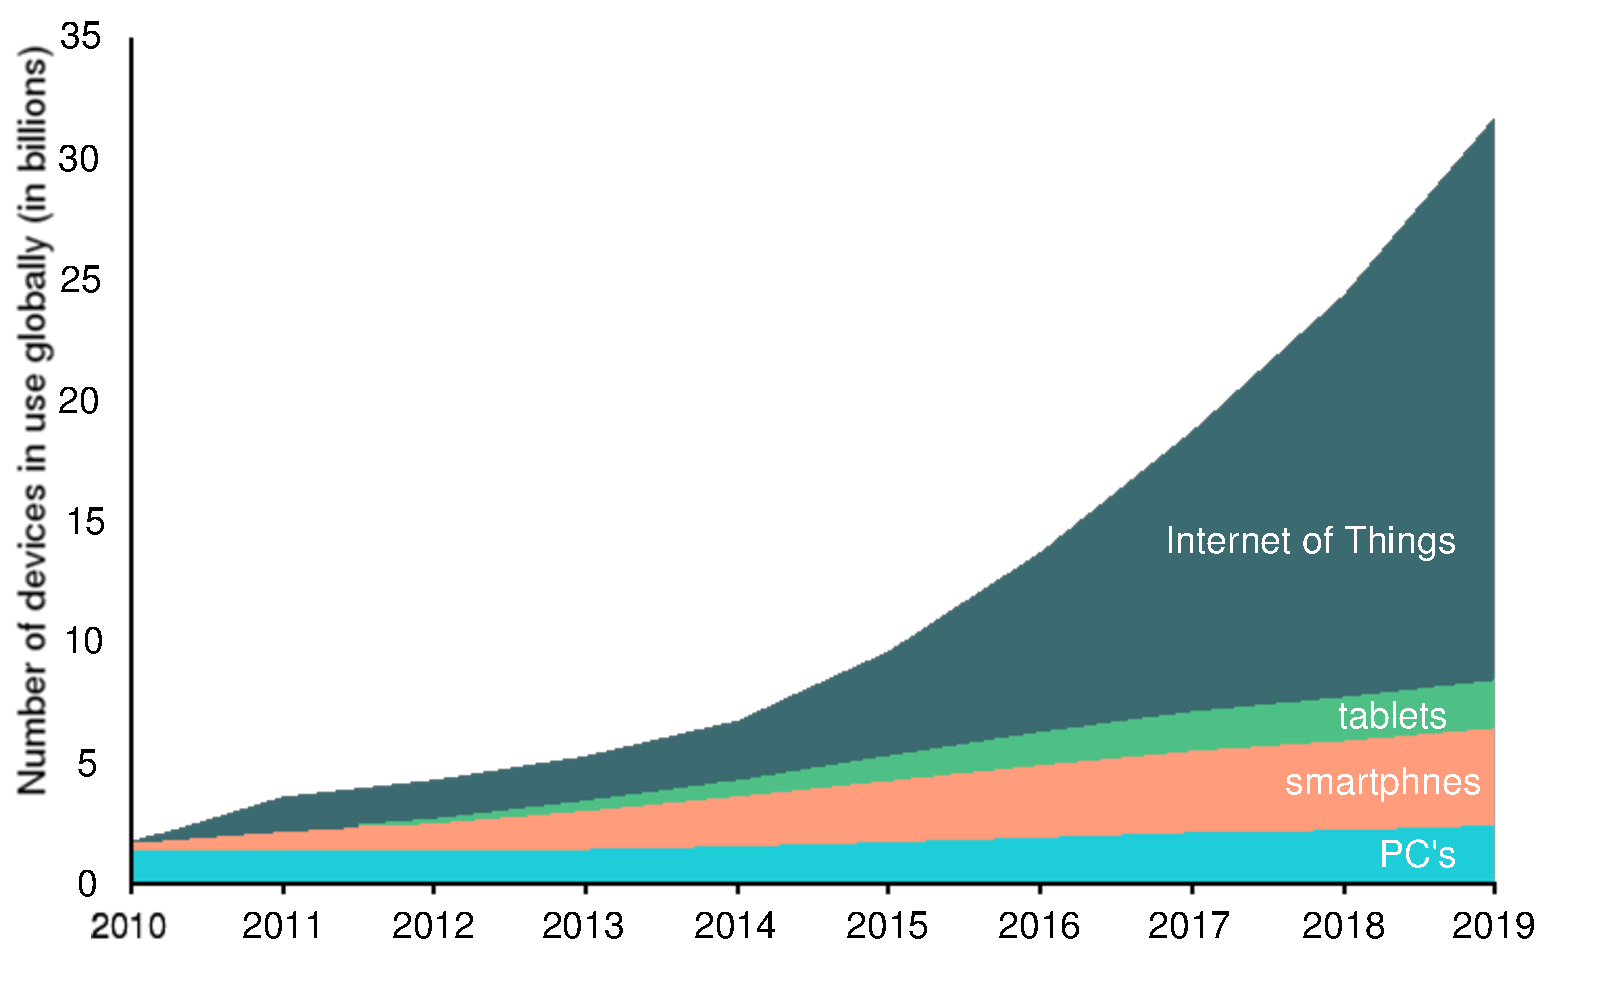
\includegraphics[width=10cm]{iot_devices}
\caption{Numero di dispositivi per anno}
\end{figure}

Questa rapida crescita ha portato alla ricerca è sviluppo di nuove soluzioni 
tecnologiche per supportare il carico di dispositivi simultaneamente connessi 
alla rete, senza avere un degrado evidente delle performance.
Per non alterare il \emph{QoS} Quality of Service della rete ed garantire costi
non elevati tecnologie come \emph{LPWAN} sono state ideate. I punti chiave per
garantire tutto ciò sono
\begin{itemize}
\item \textbf{Scalabilità}: Dato l'elevato numero di devices connessi, scenari
urbani ed industriali, la network tecnologi alla base dovrà essere estremamente
adattabile, in maniera dinamica, al carico di dispositivi connessi.
\item \textbf{Costo unitario}: Il costo del singolo modulo, dovrà essere basso
per garantire la più ampia fetta di mercato.
\item \textbf{Durata della batteria}: La maggior parte dei dispositivi sarà
alimentata tramite batteria, e la durata media e stimata di anni. 
\item \textbf{Costo computazionale}: La modulazione alla base di queste nuove
tipologie di rete, dovrà essere concepita in modo da non avere un costo
computazionale elevato.
\item \textbf{Distanza}: Un altro punto fondamentale è la possibilità di avere
comunicazioni a lunga distanza.
\end{itemize}

La rete di tipo \emph{LPWAN} è in grado di supportare tutti questi aspetti, le
principali tecnologie che già supportano questo tipo di rete son SigFox\tm,
LoRaWAN\tm, NB-IoT\tm e Weightless\tm. 

\begin{figure}[h]
\centering 
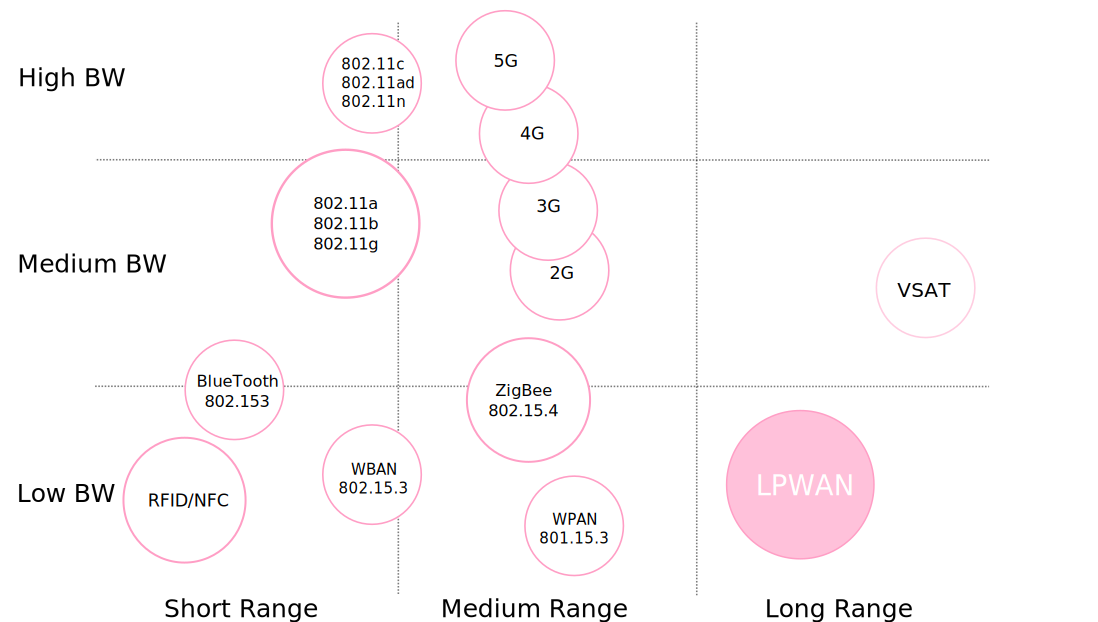
\includegraphics[width=15cm]{network_comp}
\caption{Comparazione tipologia di reti}
\end{figure}

Con questa tesi si è voluto studiare i casi applicativi della tecnologia Lora\tm
nel abito della agricoltura di precisione, utilizzando il framework open-source
Kura\tm messo a disposizione da Eurotech\tm, andando a creare un applicativo
OSGI\reg installabile nel framework. 


\mainmatter

%\section{IoT}
Sempre più spesso si parla di Internet delle cose, o IOT, con questo termine si 
intende un evoluzione delle applicazioni legate al settore mobile, al settore
della home automation e al settore embedded. 
In questo scenario ogni oggetto il
quale contiene un sensore sarà connesso ad Internet. Avvalendosi di questa
connessione , i vari dati raccolti potranno essere inviati nel cloud, dove
verranno elaborati e resi disponibili alle varie applicazioni. 
Per fare in modo che questo update avvenga, è necessario riuscire a creare una
rete di devices ,correlati nelle loro funzionalità, i quali riescano a
\emph{parlare un linguaggio comune}. \improvement{Scrivi qualcosa di decente
qui}
Il punto principale di questo
upgrade sta nel riuscire a creare una rete di devices connessi ad internet. Per
supportare e utilizzare una potenza di calcolo maggiore andando a combinare
tecniche di data analytics per estrarre le informazioni più significative. 

In
questa visione, milioni di devices saranno connessi a Internet e molto presto
milioni di milioni di devices. 

Il mercato di questi \emph{smart devices } è
in rapida crescita con una stima di 8,3 miliardi di dispositivi connessi nel
anno 2017, e di circa 20 miliardi per l'anno 2020 \cite{gartner2016}. Andando ad
creare un impatto economico compreso tra i 2.7 e i 14 trilioni di dollari. I
mercati principali saranno quelli del healt care con un introito compreso tra i
$1.1$ e i $2.5$ trilioni di dollari e il settore industriale con $2.3$ a $11.6$
trilioni di dollari.

\begin{figure}[h]
\centering 
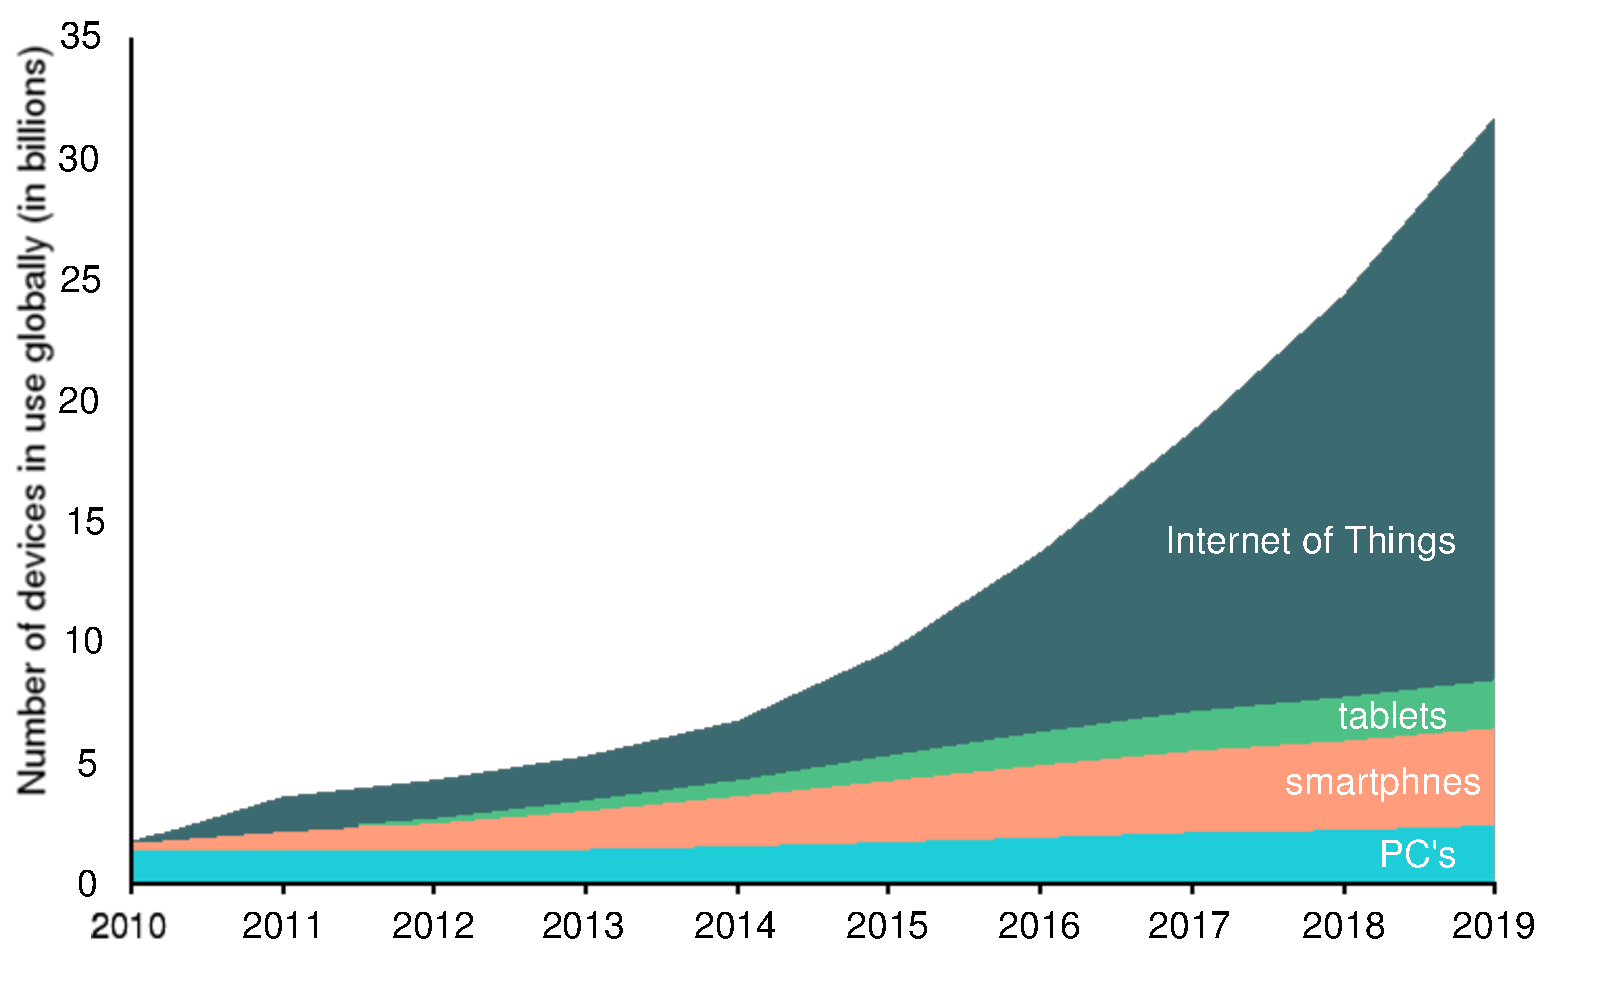
\includegraphics[width=10cm]{iot_devices}
\caption{Numero di dispositivi per anno}
\end{figure}

Questa rapida crescita ha portato alla ricerca è sviluppo di nuove soluzioni 
tecnologiche per supportare il carico di dispositivi simultaneamente connessi 
alla rete, senza avere un degrado evidente delle performance.
Per non alterare il \emph{QoS} Quality of Service della rete , hardware e
software dovranno essere rivisti insieme alla topologia di rete utilizzata. I
principali punti chiave sono

\begin{itemize}
\item \textbf{Scalabilità}: Dato l'elevato numero di devices connessi, scenari
urbani ed industriali, la network tecnologi alla base dovrà essere estremamente
adattabile, in maniera dinamica, al carico di dispositivi connessi.
\item \textbf{Costo unitario}: Il costo del singolo modulo, dovrà essere basso
per garantire la più ampia fetta di mercato.
\item \textbf{Durata della batteria}: La maggior parte dei dispositivi sarà
alimentata tramite batteria, e la durata media e stimata di anni. 
\item \textbf{Costo computazionale}: La modulazione alla base di queste nuove
tipologie di rete, dovrà essere concepita in modo da non avere un costo
computazionale elevato.
\item \textbf{Distanza}: Un altro punto fondamentale è la possibilità di avere
comunicazioni a lunga distanza.
\item \textbf{Sicurezza}: Ogni devices dovrà essere difficilmente penetrabile da
attacchi esterni.
\item \textbf{Menagment}: I vari dispositivi dovranno essere facilmente
controllabili da remoto.
\item \textbf{Fail-safe}: Il non funzionamento di devices non dovrà
compromettere l'intera infrastruttura a lui connessa. 
\end{itemize}

Vari tipi di architetture di rete sono stati proposti per realizzare questa
nuova infrastruttura. Per quanto le varie proposte si basano su tecnologie
differenti, è possibile individuare tre layer comuni 
\begin{itemize}
\item \textbf{Device layer} formato da tutti i dispositivi che collezionano dati
e sono connessi alla rete.
\item \textbf{Network layer} La struttura della rete, la quale permette di
connettere i vari devices in modo che possano scambiare i dati tra di loro o
inviarli ad un data-center.
\item \textbf{Application layer} il quale interpreta e utilizza i dati ricevuti.
\end{itemize}

Attualmente sono diversi i concorrenti che provano ad affermarsi nel settore
del IoT proponendo soluzioni diverse. Nei seguenti capitoli ci sarà un analisi
generale delle varie topologie proposte, in particolare verrà analizzata la
tecnologia Lora ed il protocolla LoraWAN.



%\chapter{LPWAN}
Data la grande varietà dei possibili scenari applicativi dell'IoT , trovare uno standard
capace di adattarsi, in modo dinamico, ad ognuno di essi, non è un compito
facile. Le tecnologie wireless tradizionali, non sono in grado di soddisfare
la dinamicità  di questo paradigma.
Già diverse soluzioni sono nate per cercare di fronteggiare questi
problemi, optando per metodi risolutivi  anche molto distanti l'uno dall'altro.
Con questo capitolo si approfondiranno le problematiche, che i nuovi standard, riguardanti il
network layer, dovranno essere in grado di risolvere.
\section{Alla base delle reti LPWAN}  
Le tecnologie wireless com ZigBee, WiFi, non sono ideate per connettere devices
alimentati a batteria distribuiti in una vasta area geografica.
Il range di queste tecnologie è limitato a poche centinaia di metri al massimo.
Tutto ciò implica che i devices, non possono essere implementati in tutti gli
ambienti, ma solo in uno spazio ristretto alla portata del segnale del gateway.
Quindi scenari quali la sicurezza sanitaria, agricoltura di precisione, logistica non
permettono l'utilizzo di questa tecnologia.
La grande copertura offerta dalle tecnologia cellulare è la ragione per la quale
è ad oggi la tecnologia più utilizzata nelle comunicazioni M2M.
Tuttavia, il continuo progresso tecnologico, sta portando l'abbandono della rete
GSM da parte degli operatori telefonici, per poter riutilizzare le bande da essa
occupata con tecnologie più innovative. In generale, la tecnologia cellulare non
garantisce una durata della batteria molto prolungata ed inoltre il costo
complessivo dei moduli cellulari è molto elevato, data la complessità delle 
forme d'onda .

Dovendo ingegnerizzare il network layer, è importante capire quali sono le
principali problematiche che le tecnologie attuali non sono in grado di colmare.

\begin{itemize}
\item \textit{Indirizzabilità}: a causa dell’elevato numero di oggetti che entrano in
gioco in IoT, la capacità di indirizzamento di IPv4 non è più suffi-
ciente. IPv4 usa 32 bit per gli indirizzi, quindi ce ne possono essere
massimo $2^{32}$ diversi. Il passaggio a IPv6 risolverà il problema, in quanto si passerà da
32 bit a 128 bit per gli indirizzi. 
\item \textit{Scalabilità}: Dato l'elevato numero di devices previsti nei scenari
urbani ed industriali, la network technology alla base della rete dovrà essere 
adattabile, in modo dinamico, al carico di dispositivi connessi.
\item \textit{"Arrive and operate”}: dispositivi mobili eventualmente aggiunti do-
po la formazione iniziale del sistema, non devono aver bisogno di
configurazione, ma devono essere in grado di stabilire connessioni
autonomamente con gli altri oggetti già presenti.
\item \textit{Costo unitario}: Il costo del end device, dovrà essere conveniente
per garantire la più ampia fetta di mercato.
\item \textit{Fonti di energia}: 
Gli oggetti nella maggior parte dei casi sono mobili, quindi non han-
no sempre la possibilità di essere collegati a una fonte di energia. Le
batterie inoltre sono pesanti e grandi.È necessario quindi andare a ridurre la quantità 
di energia richiesta dagli oggetti, andando ad aumentare il tempo di deep-sleep
.
\item \textit{Interoperabilità}: gli oggetti sono di natura diversa (per esempio
possono avere requisiti di larghezza di banda diversi, o hardware diverso).
Questo implica la necessità di standard, in modo che oggetti di tipo
diverso possano comunicare tra loro
\item \textit{Costo computazionale}: La modulazione, alla base di queste nuove
tipologie di rete, dovrà essere concepita in modo da non richiedere un costo
computazionale elevato .
\item \textit{Raggio d'azione}: La necessità di utilizzare questi devices in ambienti
difficili o rurali, rende necessario l'utilizzo di tecnologie wireless con un
raggio di azione dell'ordine di una decina di chilometri.
\item \textit{Sicurezza}: Lo scambio dei dati dovrà avvenire in maniera sicura,
implementando algoritmi di cifratura dei dati o procedure di handshaking.
\item \textit{Tolleranza ai guasti}: Il mal funzionamento  o il guasto di un
nodo della rete,  non dovrà compromettere il funzionamento dell'intera rete a lui connessa. 
\end{itemize}

\section{LPWAN}
Per colmare il gap tra tecnologie esistenti e la
necessita di connettere milioni di devices diversi, sono nate le  LPWAN
\emph{Low power wide area network}.
Le reti LPWAN rappresentano un modello  di comunicazione
innovativo, che integra le tecnologie cellulari tradizionali e quelle a corto
raggio per affrontare diverse esigenze delle applicazioni IoT. 
Le reti LPWA, andando a sacrificare il massimo throughput dei devices, ne sono in
grado di gestire un gran numero contemporaneamente, cosa che con le tecnologie
wireless tradizionali non è possibile realizzare.

\begin{figure}[ht]
    \centering 
        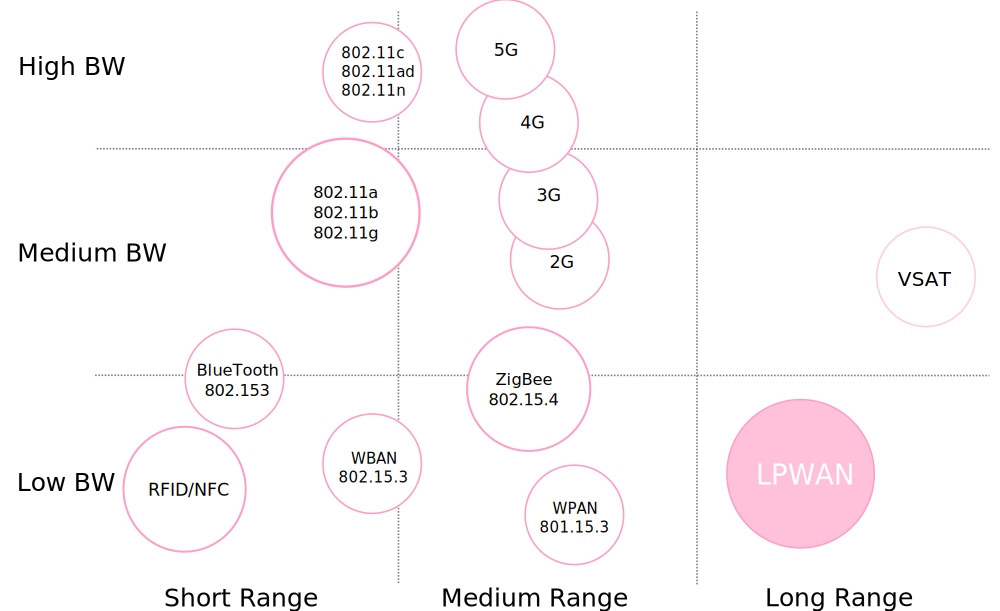
\includegraphics[width=12cm]{network-com}
    \caption{Comparazione tipologia di reti}
\end{figure}

In questo contesto, i maggiori competitor sono  NB-IoT, EC-GSM-IoT
LTE-M, SigFox e Lora. Le prime tre  sono una evoluzione delle precedenti reti
cellulari 2G,3G e 4G. Operando sulle bande di frequenza licenziate, e necessario
che ognuna di queste tecnologie sia approvata dalla 3GPP ( 3rd Generation
Partnership Project), la quale si occupa della standardizzazione dei sistemi di
telecomunicazione a livello internazionale.
All'opposto, Sigfox e Lora sono due tecnologie che operano nelle frequenze ISM
(Industrial, Scientific and Medical). Le frequenze ISM sono uno spettro radio
riservato alle applicazioni di radiocomunicazione non commerciali.

\begin{figure}[ht]
    \centering 
        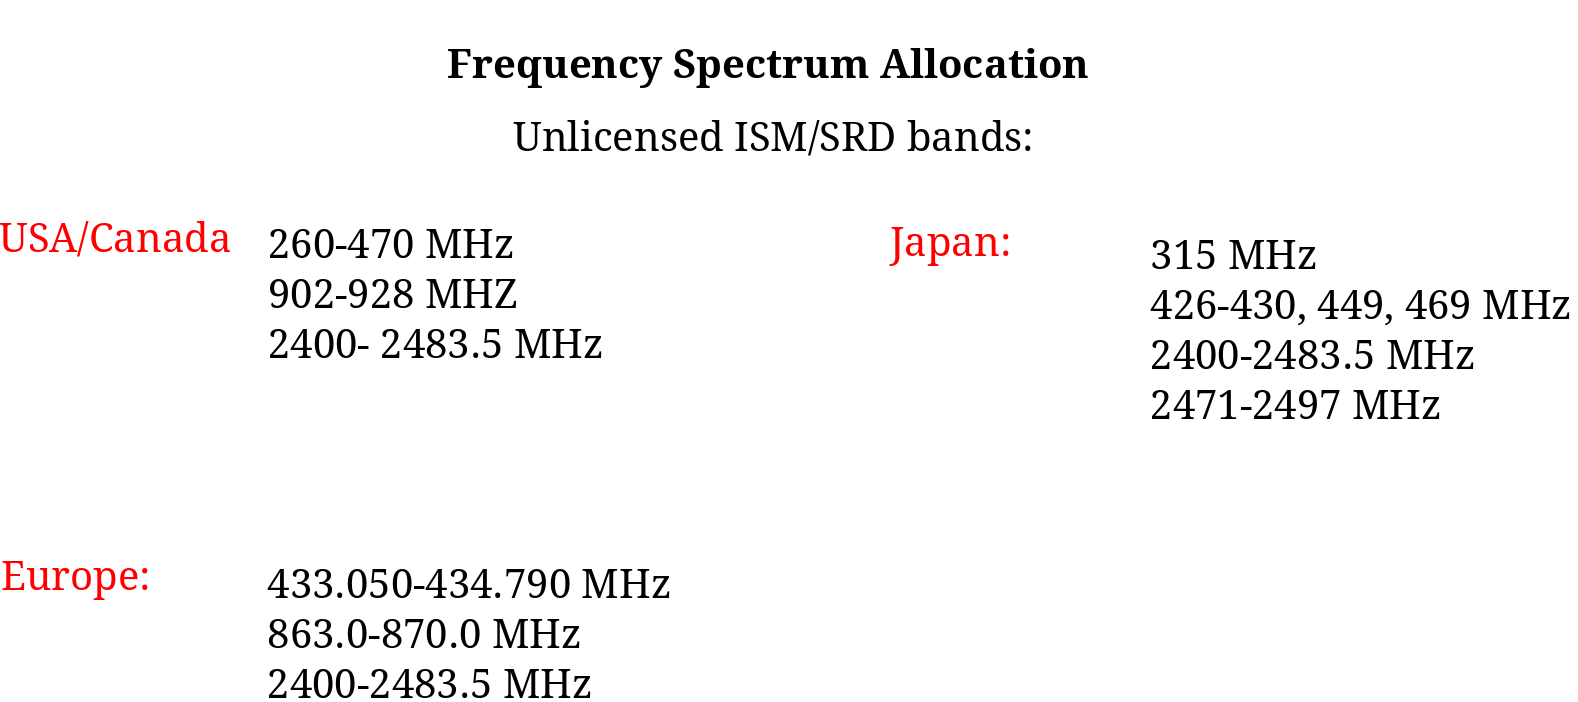
\includegraphics[width=10cm]{Orignal/freq}
    \caption{Comparazione tipologia di reti}
\end{figure}

In particolare entrambe le tecnologie operano  nella banda degli 868 [MHz]
la quale permette una potenza del segnale inviato massima pari a 14 [dbm] ed un
duty cycle inferiore al 1\%.
 
\section{NB-IoT}
Narrowband IoT (NB-IoT) o LTE Cat NB1 è uno standard certificato nella release 13 del 3GPP, la
quale riutilizza le infrastrutture già presenti, quali 2G, 3G, 4G per la rapida
realizzazione di una rete LPWA per l'IoT.
Focalizzandosi sulla durata della batteria, i moduli NB-IoT risultano avere un
costo all'unità minore del 75\% rispetto ad un normale modulo LTE.
Basato sulle frequenze licenziate, NB-IoT è in grado di
offrire tre diversi scenari di sviluppo \cite{NB-white_paper}
\begin{itemize}
\item \emph{standalone}, utilizzando qualsiasi spettro disponibile dell'
operatore.
\item \emph{guard band}, utilizzando lo spettro libero presente tra due bande
radio, per prevenire interferenze.
\item \emph{in band}, utilizzando lo stesso spettro della banda LTE.
\end{itemize}
\begin{figure}[ht]
    \centering 
        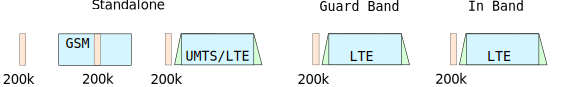
\includegraphics[width=12cm]{nb-iot}
    \caption{Modalità di funzionamento NB-IoT}
\end{figure}
L'obbiettivo che NB-IoT si prefigge è quello di mettere a disposizione una
tecnologia con una elevata copertura ed un basso data-rate. La possibilità di
riutilizzare strutture già esistenti, ed il basso costo per device , rendo
NB-IoT, una delle tecnologie che sta riscuotendo maggiore successo nel abito IoT.



\section{LTE-M}
Dalla realise 8 del 3GPP, diverse nuove tipologie di rete LTE sono disponibili.
La categoria che offre le migliori performance batteria/data-rate è la categoria
LTE Cat-M1 o LTE-M.
Questa categoria ,a differenza del NB-IoT, rispecchia lo standard LTE in pieno, 
implementando  la Frequency Division Multiplexing
(FDM) e Time Division Multiplexing (TDM). Risultando adatta per applicazioni
nelle quali è necessario l'invio di dati audio o video oppure per comunicazioni a
bassa latenza . Il data-rate raggiungibile è pari a 5Mbps in
uplink e 10 [Mbps] in downlink .  Questo tipo di connessione sarà utile
per tutte quelle applicazioni in cui è richiesta una elevata sicurezza del dato
da trasmettere, come ad esempio applicazioni di video-sorveglianza o automotive
.Questa tecnologia ,già disponibile negli Stati Uniti tramite la rete Verizon, è
in fase di roll out per molti operatori europei.

\section{EC-GSM-IoT}
EC-GSM-IoT si basa su funzionalità aggiuntive a partire da EGPRS che consentono
ad una rete GSM/EDGE di essere predisposta per fornire servizi IoT. Lo standard
è stato pensato in particolare per quei Paesi, come quelli in via di sviluppo,
dove una rete LTE non è ancora disponibile. L’occupazione spettrale di ogni
canale corrisponde a  200 kHz.  Tuttavia, al fine di dispiegare EC-GSM-IoT, si
richiede una banda utile di 2.4 MHz per permettere il frequency hopping , che,
con l’aggiunta di 2 canali di guardia di 200 kHz ciascuno agli estremi della
banda, porta l’occupazione di banda complessiva a 2.8 MHz.  La
potenza di trasmissione del Il data rate di picco raggiungibile sia in DL sia in
UL è di 491 kbps, mentre il valore mediato nominale è di 98 kbps sia in DL sia
in UL. Al fine di soddisfare i requisiti di capacità (più di 50.000 terminali in
ogni singolo settore di una cella trisettoriale). 

La figura \ref{tab:IoT_cell_comp} riassume in breve le varie caratteristiche
delle reti cellulari facenti parte della categoria LPWA
\begin{table}[h]
    \centering 
                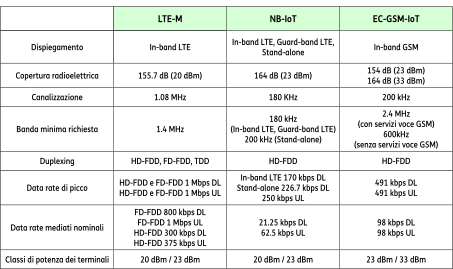
\includegraphics[width=12cm]{tim_iot}
    \caption{Comparazione reti cellulari per l'IoT}
    \label{tab:IoT_cell_comp} 
\end{table}



\section{Sigfox}
SigFox, azienda francese, sta sviluppando in partnership con altri operatori di
rete una soluzione LPWAN basata sulla sua tecnologia. Sigfox punta alla
costruzione di una rete mondiale proprietaria basata su frequenze ISM.
Correntemente SigFox è presente in Francia, Belgio, Olanda e Portogallo come
illustrato nella figura \ref{fig:Sig_covereg}.
\begin{figure}[h]
    \centering 
                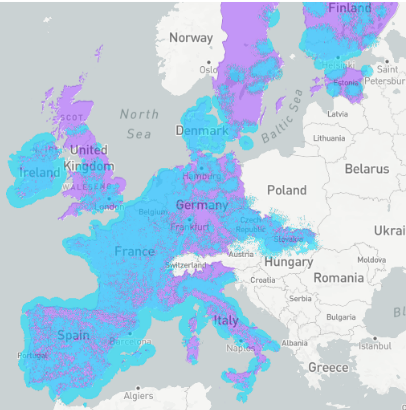
\includegraphics[width=12cm]{SigFox_covereg}
    \caption{Mappa copertura SigFox}
    \label{fig:Sig_covereg} 
\end{figure}

Gli end-devices comunicano con le varie base stations usando una modulazione (BPSK)
\emph{Binary Phase Shift Keying} con una banda di soli 100 [Hz]. 
Per via delle regolazioni vigenti nello spettro ISM, è per garantire una durata
della batteria pari ad una decina di anni, il numero massimo di messaggi
inviabili in un giorno è 140, con lunghezza del payload pari a 12 [byte] e un
throughput pari a 100 [bps]. SigFox si colloca come rete LPWAN con il minore
throughput, limitando il numero di use-case possibili. Inizialmente SigFox
supportava solo comunicazioni unidirezionali, successivamente, ha introdotto la
possibilità di avere una comunicazione bidirezionale, limitando il numero di
byte trasmissibili da gateway a devices a 4-8 bytes per giorno.

\section{LoRaWAN}
\emph{LoraWAN} è una tecnologia di modulazione wireless semi-proprietaria 
sviluppata da Semtech. Essa è composta da un layer fisico ,proprietario, che
prende il nome di \emph{Lora}\cite{LoRaCss101} , e una parte libera chiamata 
LoRaWAN\cite{LoRaWAN101} nella quale viene definito un protocollo di comunicazione, 
il quale usa LoRa come layer fisico. 
Basandosi su una tecnica di comunicazione a \emph{spread spectrum}, LoRa è in
grado di instaurare una comunicazione bidirezionale tra device e gateway.
I punti chiave dei questa tecnologia sono il grande raggio di copertura , il 
basso consumo energetico e la capacità di adattare in maniera dinamica il
data rate, il quale può variare dai 0.3 ai 50 [Kbps] a seconda dell'utilizzo. 
Come per SigFox, la tecnologia sviluppata da Semtech, si basa sulle bande ISM,
inoltre Essendo il protocollo LoRaWAN open source, si ha la possibilità di
creare delle reti pubbliche o private senza disporre di alcuna licenza, 
riducendo così il time to market di questa tecnologia.  
Progetti come \href{https://www.thethingsnetwork.org/}{The Things Network}
mirano a creare una rete LoRa ,pubblica è privata,  a livello globale.

\section{Osservazioni}
In questo mercato frammentato, non è semplice capire quale tecnologia sia adatta
a ricoprire una data applicazione. Essendo questi standard molto giovani, è
complicato comprendere le reali potenzialità di ognuna di queste soluzioni.
Quello che è possibile prevedere, sarà un incremento esponenziale di device che
stanno alla base della piramide in figura \ref{fig:pyramid}, devices i quali
potranno essere utilizzati in innumerevoli settori, non ancora esplorati dalle
tecnologie attuali, come per esempio i contatori della dell'acqua, applicazioni
per l'agricoltura di precisione e così via. 

\begin{figure}[ht]
    \centering 
                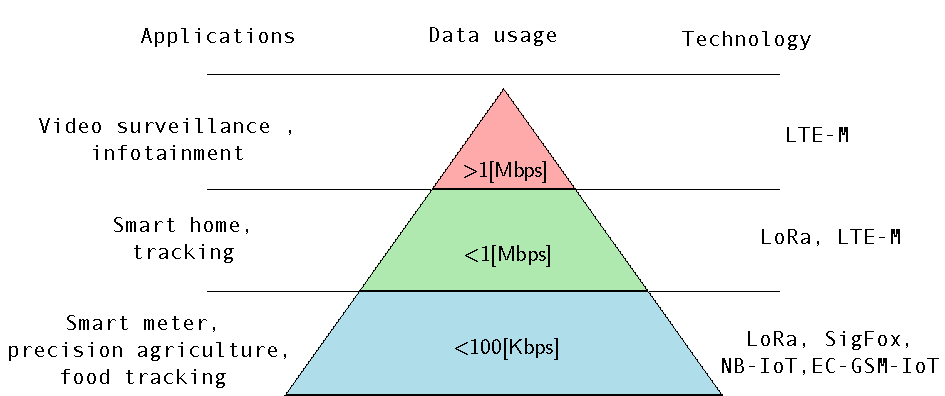
\includegraphics[width=12cm]{pyramid}
    \caption{Capacità delle reti LPWA}
    \label{fig:pyramid} 
\end{figure}

\pagebreak
Per le aziende, che si apprestano ad investire sul mondo dell'IoT, la scelta
della corretta tecnologia su cui andare a sviluppare i loro servizi non risulta
semplice, in quanto, fattori quali sicurezza, aggiornamenti software,
affidabilità devono essere ancora testati a pieno. Con la figura
\ref{fig:feature_comp} si vuole riassumere in breve i punti chiave delle
tecnologie appena trattate.

\begin{figure}[ht]
    \centering 
                \includegraphics[width=9cm]{Comparsion_no_line}
    \caption{Comparazione feature reti LPWAN}
    \label{fig:feature_comp} 
\end{figure}

Nel prossimo capitolo verrà analizzata in dettaglio la soluzione che Semtech
propone, approfondendo il layer fisico \emph{Lora} e la struttura del protocollo
LoRaWAN.


%\include{Tex_Files/Chapters/Conclusioni}


%\appendix
  
%\include{appendici}

\backmatter

\include{biblio}

 %\printindex % se si fa l'indice analitico.

\end{document}
